\subsection{Setup}\label{sec:setup}
The tests are, as mentioned in Section \ref{sec:groupgeneration}, going to be performed on groups with member sizes of 4, 8, 12, 16, 20, and 40, and there are going to be 1000 random generated groups of each size. Throughout these tests we have decided to assign $k$ to have the size 10.  
\begin{figure}[h]
\centering
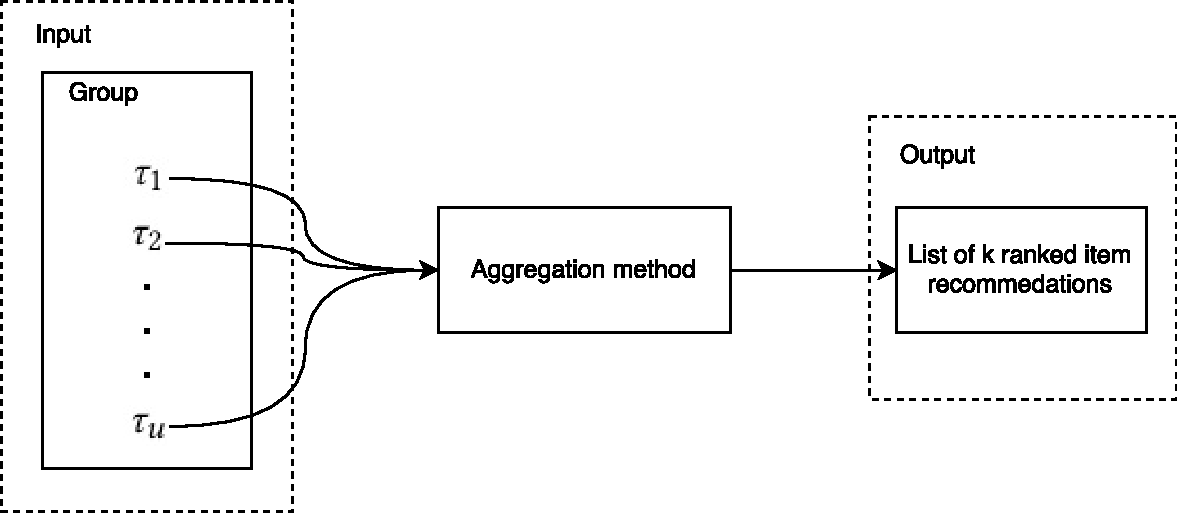
\includegraphics[scale=.4]{graphics/setup}
\caption{Test setup}\label{fig:composition}
\end{figure}
\subsubsection{T-test}
We made paired t-tests for all methods. Each method is compared with each of the other methods for all measures. The t-test outputs a p-value, which is the probability that the difference between two sets of results is coincidental. At $0.05$ or lower, it is considered that there is statistically significant difference in the means of the two sets.\note{Citation}
\subsubsection{Ranking Measures}
As mentioned we are going to used nDCG, Rating nDCG, KTD and SFD. The way we are going to present the results of these tests are by finding the average scores for the test across a group size. What this means is the we first find an average score for a group and when having the average for all the groups, we find a global average between all groups of a given size. 